%% bare_conf.tex
%% V1.4b
%% 2015/08/26
%% by Michael Shell
%% See:
%% http://www.michaelshell.org/
%% for current contact information.
%%
%% This is a skeleton file demonstrating the use of IEEEtran.cls
%% (requires IEEEtran.cls version 1.8b or later) with an IEEE
%% conference paper.
%%
%% Support sites:
%% http://www.michaelshell.org/tex/ieeetran/
%% http://www.ctan.org/pkg/ieeetran
%% and
%% http://www.ieee.org/

%%*************************************************************************
%% Legal Notice:
%% This code is offered as-is without any warranty either expressed or
%% implied; without even the implied warranty of MERCHANTABILITY or
%% FITNESS FOR A PARTICULAR PURPOSE! 
%% User assumes all risk.
%% In no event shall the IEEE or any contributor to this code be liable for
%% any damages or losses, including, but not limited to, incidental,
%% consequential, or any other damages, resulting from the use or misuse
%% of any information contained here.
%%
%% All comments are the opinions of their respective authors and are not
%% necessarily endorsed by the IEEE.
%%
%% This work is distributed under the LaTeX Project Public License (LPPL)
%% ( http://www.latex-project.org/ ) version 1.3, and may be freely used,
%% distributed and modified. A copy of the LPPL, version 1.3, is included
%% in the base LaTeX documentation of all distributions of LaTeX released
%% 2003/12/01 or later.
%% Retain all contribution notices and credits.
%% ** Modified files should be clearly indicated as such, including  **
%% ** renaming them and changing author support contact information. **
%%*************************************************************************


% *** Authors should verify (and, if needed, correct) their LaTeX system  ***
% *** with the testflow diagnostic prior to trusting their LaTeX framework ***
% *** with production work. The IEEE's font choices and paper sizes can   ***
% *** trigger bugs that do not appear when using other class files.       ***                          ***
% The testflow support page is at:
% http://www.michaelshell.org/tex/testflow/


\label{beginning of document}
\documentclass[conference]{IEEEtran}
% Some Computer Society conferences also require the compsoc mode option,
% but others use the standard conference format.
%
% If IEEEtran.cls has not been installed into the LaTeX system files,
% manually specify the path to it like:
% \documentclass[conference]{../sty/IEEEtran}

\usepackage{graphicx}
	\graphicspath{{images/}} 
\renewcommand\IEEEkeywordsname{Keywords}
\usepackage{hyperref}
	\hypersetup{colorlinks=true,allcolors=blue}
\usepackage{hypcap}
\usepackage{subfig}
\usepackage{listings}
	\lstset{
  		basicstyle=\ttfamily\scriptsize,
  		frame=single,
  		breaklines=true,
  		numbers=left,
  		xleftmargin=2.5em,
  		framexleftmargin=0em,
  		emph={
        	class, extends, operation, abstract,
        	context, constraint, check,
        	for, if, return, true, and, ref,
        	message, in, package, val, attr, 
        	@link, @node, @compartment,
        	@namespace, @diagram
    	},
    	emphstyle=\textbf
	}
	\lstdefinestyle{interfaces}{
  		float=t
	}

% Some very useful LaTeX packages include:
% (uncomment the ones you want to load)


% *** MISC UTILITY PACKAGES ***
%
%\usepackage{ifpdf}
% Heiko Oberdiek's ifpdf.sty is very useful if you need conditional
% compilation based on whether the output is pdf or dvi.
% usage:
% \ifpdf
%   % pdf code
% \else
%   % dvi code
% \fi
% The latest version of ifpdf.sty can be obtained from:
% http://www.ctan.org/pkg/ifpdf
% Also, note that IEEEtran.cls V1.7 and later provides a builtin
% \ifCLASSINFOpdf conditional that works the same way.
% When switching from latex to pdflatex and vice-versa, the compiler may
% have to be run twice to clear warning/error messages.






% *** CITATION PACKAGES ***
%
%\usepackage{cite}
% cite.sty was written by Donald Arseneau
% V1.6 and later of IEEEtran pre-defines the format of the cite.sty package
% \cite{} output to follow that of the IEEE. Loading the cite package will
% result in citation numbers being automatically sorted and properly
% "compressed/ranged". e.g., [1], [9], [2], [7], [5], [6] without using
% cite.sty will become [1], [2], [5]----[7], [9] using cite.sty. cite.sty's
% \cite will automatically add leading space, if needed. Use cite.sty's
% noadjust option (cite.sty V3.8 and later) if you want to turn this off
% such as if a citation ever needs to be enclosed in parenthesis.
% cite.sty is already installed on most LaTeX systems. Be sure and use
% version 5.0 (2009-03-20) and later if using hyperref.sty.
% The latest version can be obtained at:
% http://www.ctan.org/pkg/cite
% The documentation is contained in the cite.sty file itself.






% *** GRAPHICS RELATED PACKAGES ***
%
\ifCLASSINFOpdf
  % \usepackage[pdftex]{graphicx}
  % declare the path(s) where your graphic files are
  % \graphicspath{{../pdf/}{../jpeg/}}
  % and their extensions so you won't have to specify these with
  % every instance of \includegraphics
  % \DeclareGraphicsExtensions{.pdf,.jpeg,.png}
\else
  % or other class option (dvipsone, dvipdf, if not using dvips). graphicx
  % will default to the driver specified in the system graphics.cfg if no
  % driver is specified.
  % \usepackage[dvips]{graphicx}
  % declare the path(s) where your graphic files are
  % \graphicspath{{../eps/}}
  % and their extensions so you won't have to specify these with
  % every instance of \includegraphics
  % \DeclareGraphicsExtensions{.eps}
\fi
% graphicx was written by David Carlisle and Sebastian Rahtz. It is
% required if you want graphics, photos, etc. graphicx.sty is already
% installed on most LaTeX systems. The latest version and documentation
% can be obtained at: 
% http://www.ctan.org/pkg/graphicx
% Another good source of documentation is "Using Imported Graphics in
% LaTeX2e" by Keith Reckdahl which can be found at:
% http://www.ctan.org/pkg/epslatex
%
% latex, and pdflatex in dvi mode, support graphics in encapsulated
% postscript (.eps) format. pdflatex in pdf mode supports graphics
% in .pdf, .jpeg, .png and .mps (metapost) formats. Users should ensure
% that all non-photo figures use a vector format (.eps, .pdf, .mps) and
% not a bitmapped formats (.jpeg, .png). The IEEE frowns on bitmapped formats
% which can result in "jaggedy"/blurry rendering of lines and letters as
% well as large increases in file sizes.
%
% You can find documentation about the pdfTeX application at:
% http://www.tug.org/applications/pdftex





% *** MATH PACKAGES ***
%
%\usepackage{amsmath}
% A popular package from the American Mathematical Society that provides
% many useful and powerful commands for dealing with mathematics.
%
% Note that the amsmath package sets \interdisplaylinepenalty to 10000
% thus preventing page breaks from occurring within multiline equations. Use:
%\interdisplaylinepenalty=2500
% after loading amsmath to restore such page breaks as IEEEtran.cls normally
% does. amsmath.sty is already installed on most LaTeX systems. The latest
% version and documentation can be obtained at:
% http://www.ctan.org/pkg/amsmath





% *** SPECIALIZED LIST PACKAGES ***
%
%\usepackage{algorithmic}
% algorithmic.sty was written by Peter Williams and Rogerio Brito.
% This package provides an algorithmic environment fo describing algorithms.
% You can use the algorithmic environment in-text or within a figure
% environment to provide for a floating algorithm. Do NOT use the algorithm
% floating environment provided by algorithm.sty (by the same authors) or
% algorithm2e.sty (by Christophe Fiorio) as the IEEE does not use dedicated
% algorithm float types and packages that provide these will not provide
% correct IEEE style captions. The latest version and documentation of
% algorithmic.sty can be obtained at:
% http://www.ctan.org/pkg/algorithms
% Also of interest may be the (relatively newer and more customizable)
% algorithmicx.sty package by Szasz Janos:
% http://www.ctan.org/pkg/algorithmicx




% *** ALIGNMENT PACKAGES ***
%
%\usepackage{array}
% Frank Mittelbach's and David Carlisle's array.sty patches and improves
% the standard LaTeX2e array and tabular environments to provide better
% appearance and additional user controls. As the default LaTeX2e table
% generation code is lacking to the point of almost being broken with
% respect to the quality of the end results, all users are strongly
% advised to use an enhanced (at the very least that provided by array.sty)
% set of table tools. array.sty is already installed on most systems. The
% latest version and documentation can be obtained at:
% http://www.ctan.org/pkg/array


% IEEEtran contains the IEEEeqnarray family of commands that can be used to
% generate multiline equations as well as matrices, tables, etc., of high
% quality.




% *** SUBFIGURE PACKAGES ***
%\ifCLASSOPTIONcompsoc
%  \usepackage[caption=false,font=normalsize,labelfont=sf,textfont=sf]{subfig}
%\else
%  \usepackage[caption=false,font=footnotesize]{subfig}
%\fi
% subfig.sty, written by Steven Douglas Cochran, is the modern replacement
% for subfigure.sty, the latter of which is no longer maintained and is
% incompatible with some LaTeX packages including fixltx2e. However,
% subfig.sty requires and automatically loads Axel Sommerfeldt's caption.sty
% which will override IEEEtran.cls' handling of captions and this will result
% in non-IEEE style figure/table captions. To prevent this problem, be sure
% and invoke subfig.sty's "caption=false" package option (available since
% subfig.sty version 1.3, 2005/06/28) as this is will preserve IEEEtran.cls
% handling of captions.
% Note that the Computer Society format requires a larger sans serif font
% than the serif footnote size font used in traditional IEEE formatting
% and thus the need to invoke different subfig.sty package options depending
% on whether compsoc mode has been enabled.
%
% The latest version and documentation of subfig.sty can be obtained at:
% http://www.ctan.org/pkg/subfig




% *** FLOAT PACKAGES ***
%
%\usepackage{fixltx2e}
% fixltx2e, the successor to the earlier fix2col.sty, was written by
% Frank Mittelbach and David Carlisle. This package corrects a few problems
% in the LaTeX2e kernel, the most notable of which is that in current
% LaTeX2e releases, the ordering of single and double column floats is not
% guaranteed to be preserved. Thus, an unpatched LaTeX2e can allow a
% single column figure to be placed prior to an earlier double column
% figure.
% Be aware that LaTeX2e kernels dated 2015 and later have fixltx2e.sty's
% corrections already built into the system in which case a warning will
% be issued if an attempt is made to load fixltx2e.sty as it is no longer
% needed.
% The latest version and documentation can be found at:
% http://www.ctan.org/pkg/fixltx2e


%\usepackage{stfloats}
% stfloats.sty was written by Sigitas Tolusis. This package gives LaTeX2e
% the ability to do double column floats at the bottom of the page as well
% as the top. (e.g., "\begin{figure*}[!b]" is not normally possible in
% LaTeX2e). It also provides a command:
%\fnbelowfloat
% to enable the placement of footnotes below bottom floats (the standard
% LaTeX2e kernel puts them above bottom floats). This is an invasive package
% which rewrites many portions of the LaTeX2e float routines. It may not work
% with other packages that modify the LaTeX2e float routines. The latest
% version and documentation can be obtained at:
% http://www.ctan.org/pkg/stfloats
% Do not use the stfloats baselinefloat ability as the IEEE does not allow
% \baselineskip to stretch. Authors submitting work to the IEEE should note
% that the IEEE rarely uses double column equations and that authors should try
% to avoid such use. Do not be tempted to use the cuted.sty or midfloat.sty
% packages (also by Sigitas Tolusis) as the IEEE does not format its papers in
% such ways.
% Do not attempt to use stfloats with fixltx2e as they are incompatible.
% Instead, use Morten Hogholm'a dblfloatfix which combines the features
% of both fixltx2e and stfloats:
%
% \usepackage{dblfloatfix}
% The latest version can be found at:
% http://www.ctan.org/pkg/dblfloatfix




% *** PDF, URL AND HYPERLINK PACKAGES ***
%
%\usepackage{url}
% url.sty was written by Donald Arseneau. It provides better support for
% handling and breaking URLs. url.sty is already installed on most LaTeX
% systems. The latest version and documentation can be obtained at:
% http://www.ctan.org/pkg/url
% Basically, \url{my_url_here}.




% *** Do not adjust lengths that control margins, column widths, etc. ***
% *** Do not use packages that alter fonts (such as pslatex).         ***
% There should be no need to do such things with IEEEtran.cls V1.6 and later.
% (Unless specifically asked to do so by the journal or conference you plan
% to submit to, of course. )


% correct bad hyphenation here
\hyphenation{op-tical net-works semi-conduc-tor}


\begin{document}
%
% paper title
% Titles are generally capitalized except for words such as a, an, and, as,
% at, but, by, for, in, nor, of, on, or, the, to and up, which are usually
% not capitalized unless they are the first or last word of the title.
% Linebreaks \\ can be used within to get better formatting as desired.
% Do not put math or special symbols in the title.
\title{Towards Model-Driven\\Gamified Software Modelling Learning}


% author names and affiliations
% use a multiple column layout for up to three different
% affiliations
\author{\IEEEauthorblockN{Alfa Yohannis\IEEEauthorrefmark{1}, Dimitris Kolovos, Fiona Polack}
\IEEEauthorblockA{Department of Computer Science\\
University of York\\
York, United Kingdom\\
Email: \IEEEauthorrefmark{1}ary506@york.ac.uk}}

% conference papers do not typically use \thanks and this command
% is locked out in conference mode. If really needed, such as for
% the acknowledgment of grants, issue a \IEEEoverridecommandlockouts
% after \documentclass

% for over three affiliations, or if they all won't fit within the width
% of the page, use this alternative format:
% 
%\author{\IEEEauthorblockN{Michael Shell\IEEEauthorrefmark{1},
%Homer Simpson\IEEEauthorrefmark{2},
%James Kirk\IEEEauthorrefmark{3}, 
%Montgomery Scott\IEEEauthorrefmark{3} and
%Eldon Tyrell\IEEEauthorrefmark{4}}
%\IEEEauthorblockA{\IEEEauthorrefmark{1}School of Electrical and Computer Engineering\\
%Georgia Institute of Technology,
%Atlanta, Georgia 30332--0250\\ Email: see http://www.michaelshell.org/contact.html}
%\IEEEauthorblockA{\IEEEauthorrefmark{2}Twentieth Century Fox, Springfield, USA\\
%Email: homer@thesimpsons.com}
%\IEEEauthorblockA{\IEEEauthorrefmark{3}Starfleet Academy, San Francisco, California 96678-2391\\
%Telephone: (800) 555--1212, Fax: (888) 555--1212}
%\IEEEauthorblockA{\IEEEauthorrefmark{4}Tyrell Inc., 123 Replicant Street, Los Angeles, California 90210--4321}}




% use for special paper notices
%\IEEEspecialpapernotice{(Invited Paper)}




% make the title area
\maketitle

% As a general rule, do not put math, special symbols or citations
% in the abstract
\begin{abstract}
\label{abstract}
Motivated by the success of gameful approaches in different fields, this research harnesses the engaging nature of games combined with the effectiveness of pedagogy and the automation of Model-Driven Engineering to propose a framework for model-driven gamified software modelling learning. The framework allows tutors to create software modelling learning activities, and to generate software modelling learning games for learners to play. This paper presents the motivation behind the framework, analyses the main dimensions of our work, and presents an early prototype using an example. Two forms of assessments are presented as the evaluation of the framework.
\end{abstract}

% no keywords
\begin{IEEEkeywords} 
model-driven, games, software modelling, learning
\end{IEEEkeywords}



% For peer review papers, you can put extra information on the cover
% page as needed:
% \ifCLASSOPTIONpeerreview
% \begin{center} \bfseries EDICS Category: 3-BBND \end{center}
% \fi
%
% For peerreview papers, this IEEEtran command inserts a page break and
% creates the second title. It will be ignored for other modes.
\IEEEpeerreviewmaketitle

\section{Introduction}
Gameful approaches, whether gamification \cite{stieglitz2016gamification}, serious games \cite{dorner2016serious}, or digital game-based learning \cite{san2015games}, have proven to have significant impact for a variety of purposes, such as learning, skill acquisitions, engagement, psychological support, and socialisation. \cite{connolly2012systematic, hamari2014does}. Duolingo\footnote{\url{https://www.duolingo.com}}, an application for learning new languages, and Re-mission\footnote{\url{http://www.re-mission.net}}, a game to learn to deal with cancer, are two popular examples of gameful approaches. The application of a gameful approach to software engineering has not been studied extensively \cite{Pedreira2015}, and even less so in the context of software modelling learning. 

Some works that use gameful approach in software modelling learning are 
\cite{Groenewegen2010, Stikkolorum2014, Richardsen2014, Ionita2015,  de2015gamification}. Each addresses a different problem using very specific approaches and game elements. In this paper we present a more generic approach for addressing software modelling learning so that tutors do not need to develop games from scratch to deal with each topic. We propose a framework for teaching and learning software modelling--a framework for tutors to create software modelling learning games at a high level of abstraction, which can be transformed to generate software modelling learning games for learners to play and learn with.

The paper starts with the introduction to the motivation of our work. Section \ref{Problem Analysis} reviews the core dimensions of the problem of software modelling gamification. In Section \ref{Solution Overview}, an overview of our solution is described. Section \ref{Demonstration} demonstrates use of the framework from the creation to the playing of a modelling game. Section \ref{Evaluation Plans} presents the plan to evaluate the framework. Section \ref{Related Work} summarises previous work related to this research. Finally, conclusions and directions for future work are presented in Section \ref{Conclusions}.

\section{Problem Analysis}
\label{Problem Analysis}
The main challenge addressed in this work is transforming software modelling learning into gameful activities. Given that there are different types of modelling languages (e.g. graphical, textual, projectional, tree-based) and types of games (continuous vs. level-based, real-time vs. turn-based, single-player vs. multi-player), at this stage it is worth noting that our study is limited to level-based single-player games for languages with a 2D graphical syntax. For this style of game, we have identified the following concerns and challenges.

\subsubsection{Challenge and Support}
\label{Challenge and Support}
In order to engage continuously in a learning activity, learners have to be introduced to more difficult challenges as their competence grows \cite{csikszentmihalyi2014toward}. Also, learners need to be given support which should be gradually reduced until they are capable enough to solve the challenge by themselves, as suggested by scaffolded learning \cite{wood1976role, vygotsky1978mind}. Support can be provided through procedural instructions, clues, examples, small activities, and partial pre-made models. The tutor needs to be able to design such facilities as part of the learning activity design. 

\subsubsection{Game Mechanics} 
\label{Game Mechanics} 
Gameful design method \cite{deterding2015lens} suggests that, to apply gamification, the core activity should be identified before gameful modification can be implemented. Modelling using graphical modelling languages, such as constructing and modifying diagrams, mainly involves design, editing, and planning activities. The LM-GM framework \cite{arnab2015mapping} mentions these activities as game mechanics that can be used for learning, specifically to address the \emph{creating} category in Bloom's taxonomy \cite{krathwohl2002revision}. Thus, the activity of constructing and modifying diagrams can be used as game mechanics as well, as it also involves design, editing, and planning activities as in design, editing, and planning game mechanics.

As for gameplay, learners are asked to construct or modify diagrams so that the diagrams become consistent with a given problem description and instruction. They do not always have to start with an empty canvas, but could start from existing, incomplete diagrams that are pre-made to help them focus on the core concepts and activities being taught \cite{deterding2015lens}. We name this kind of play as `construction gameplay'. Other forms of play can be supported. For example, learners can be provided with a problem description and a number of diagrams reflecting candidate solutions and asked to select the correct solution(s). In another form, learners can be given a diagram and a number of statements in natural language and choose the correct interpretation(s) or statement(s). We call these two forms of play `multiple-choice gameplay'. Tutors need to be able to define multiple levels of different gameplays and link them up to assemble complex games. 

For construction gameplay, a graphical editor through which the user can construct/modify solutions is needed. Ideally, the editor should be fully integrated into the game to provide live feedback and an immersive experience. An alternative is to ask the user to create/edit models in an existing modelling tool and upload them to the game. To simplify the definition of graphical editors embedded in the game, a standardised way to define the abstract and graphical syntaxes of supported languages is required. 

\subsubsection{Assessing Correctness} 
\label{Assessing Correctness} 
There are several ways to assess consistency and correctness for the construction gameplay. One option is to require that the provided diagram is a 1:1 match with a reference solution given by the game designer. A more relaxed approach is only to require that the provided solution satisfies a number of constraints. Another option is to require some form of semantic equivalence between the two models (e.g. class diagrams that are consistent with an object diagram). 

\subsubsection{Rewards}
\label{Rewards}
Rewards are a major element of learning games, allowing users to develop a sense of achievement, show off their new skills, and compare themselves against other users, etc. So far, we have selected two types of rewards, positive reinforcement and achievements. Positive reinforcement can have the form of sounds, visual effects, or motivating messages to give feedback to players. Positive reinforcement is intended to improve the self-efficacy of players by letting them know whether their actions are in the right direction, so they can decide and continue to execute their next actions \cite{richter2015studying}. Another reward is a list of a learner's achievements, which can act like a `CV' for a learner. It records the names, types, and numbers of levels and learning activities that they have been completed. Since a learning activity usually addresses a concept in software modelling, this could be used as a base to claim that the learners have acquired the competence -- knowledge and skill -- for that concept \cite{richter2015studying}. Building a learner's competence also means strengthening their intrinsic motivation \cite{ryan2017self} and make game playing  activities important to them \cite{nicholson2015recipe}.

\section{Solution Overview}
\label{Solution Overview}
A web-based prototype of the framework has been developed to facilitate the design and implementation of software modelling games in line with the concerns discussed in the Problem Analysis (Section \ref{Problem Analysis}). The prototype implements a metamodel-annotation-based approach for defining the concrete syntax of the targeted modelling languages. Metamodels are defined in Ecore \cite{steinberg2008emf} and their concrete syntax is specified using Eugenia-like annotations\footnote{\url{http://www.eclipse.org/epsilon/doc/articles/eugenia-gmf-tutorial/}} \cite{kolovos2015eugenia}. Tutors can define a class as the root object of a metamodel (annotated with {\fontfamily{pcr}\selectfont @diagram}), denote classes to appears as nodes ({\fontfamily{pcr}\selectfont @node}) or links ({\fontfamily{pcr}\selectfont @link}), and denote a containment references to appear as compartments where elements of the type of the reference can be nested/spatially contained ({\fontfamily{pcr}\selectfont @compartment}). The instances of the annotated classes are displayed as visual elements in a web-based graphical editor built upon the MxGraph framework\footnote{\url{https://jgraph.github.io/mxgraph/}}. Tutors can adjust the appearance of the visual elements by setting the values of appropriate annotation parameters (for example, see Listing \ref{metamodel} and Fig. \ref{example-01}-\ref{example-03} for the visual elements produced). A complete list of the supported annotations and parameters cannot be presented here due to space limitations, however, an indicative subset of them is illustrated in the example demonstrated in Section \ref{Demonstration}.

\begin{figure}[t!]
\centering
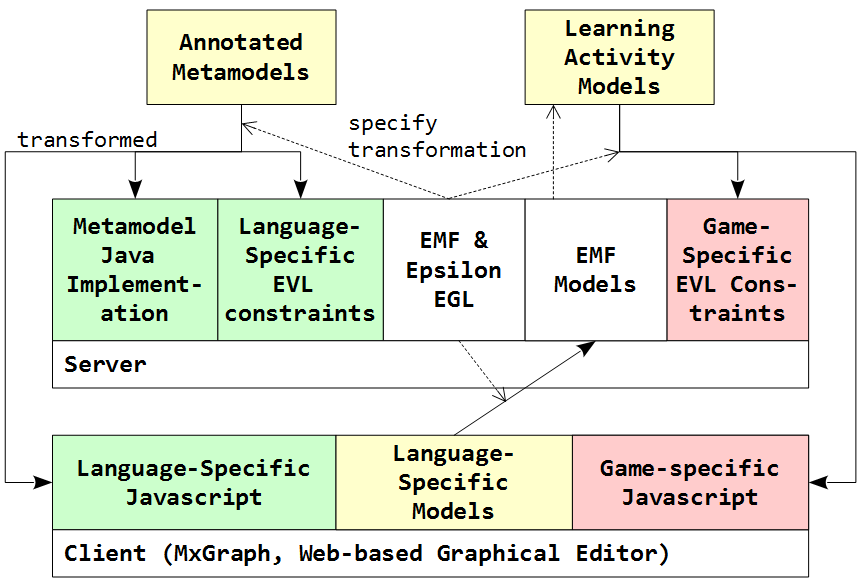
\includegraphics[width=\linewidth]{artefacts}
\caption{The framework's artefacts of the gamified software modelling learning.}
\label{artefacts}
\end{figure}


An annotated metamodel is then transformed using Epsilon EGL \cite{kolovos2010epsilon} and EMF \cite{steinberg2008emf} to generate its Java implementation code for further model management operations on the server, such as model validation and transformation (Fig. \ref{artefacts}). The transformation also produces Javascript that implements a language-specific web-based graphical editor built on top of the MxGraph framework. After the generation, tutors can create language-specific models using this editor and validate them using language-specific EVL \cite{kolovos2006eclipse} constraints (Fig. \ref{artefacts}). The models (the EMF models in Fig. \ref{artefacts}) can be used as base models in construction gameplay and are required as candidate solutions, and as diagrams to be selected and interpreted by learners in multiple-choice gameplay (the Game Mechanics concern in Subsection \ref{Game Mechanics} is addressed).  

A modelling language has also been defined to design and link up different types of levels (see Fig. \ref{laml} for its metamodel). We name the models constructed by this modelling language, \emph{learning activity models} (for example, see Fig. \ref{eoml}). Currently, elements that are supported by the learning activity modelling language are activity, objective, model, start, end, transition, and link. The activity element represents an activity in a learning process (in the transformation that follows each activity is transformed to a level). In an activity, tutors need to define \emph{lesson} (description of the topic being taught), \emph{instruction} (direction to complete the activity), the name of the target metamodel, and a set of \emph{objectives}(elements to describe targets/conditions that learners have to meet in order to complete an activity). 

A \emph{model} is an element that refers to an existing model (the EMF models in Fig. \ref{artefacts}) created by tutors or a target model that will be produced by an activity. The referred model is used as the base model when learners start an activity, so they don't have to create the referred model from the scratch. The \emph{start} and \emph{end} elements indicate where a learning activity should start and end. A \emph{transition} element is a directed edge that connects one activity to another, and \emph{link} element is also a directed edge that connects a model to an activity and \textit{vice versa}. Facilitating tutors to create different learning activity models as well as to construct different models as base models for various visual modelling languages allows tutors to adjust the difficulty and support provided (the Challenge and Support concern in Subsection \ref{Challenge and Support} is addressed). 

Learning activity models are consumed by a model-to-text transformation to generate game-specific Javascript that implements a complete playable game (Fig. \ref{artefacts}). The framework can host a number of generated games and provides features such as authentication, progress management, learning activity inventory, model inventory, etc.  

The generation also produces a game-specific EVL skeleton (Fig. \ref{artefacts}) for each level where tutors can define constraints and operations used for validation, to determine whether the level has been completed and all its objectives have been met. Currently, only the construction gameplay is supported at each level, and the correctness of solutions is assessed using the EVL constraints. So far with EVL, tutors can create rules to perform 1:1 match validation between a diagram and a reference solution and to check that a solution satisfies a number of constraints (the Assessing Correctness concern in Subsection \ref{Assessing Correctness} is addressed). The multiple-choice gameplay (Subsection \ref{Game Mechanics}), and other validation approaches (Subsection \ref{Assessing Correctness}), as well as reward mechanisms (Subsection \ref{Rewards}), are in development. 


\section{Demonstration}
\label{Demonstration}
In this section, an example is presented to demonstrate the use of the framework in a game that introduces the concept of substates in UML statechart modelling. Learners are assumed to already understand the concepts of state, transition, start state, and final state. The following subsectionspresent the different stages of the lifecycle of the game from definition to full use in game play.
 
\subsection{Define Statechart Metamodel}
For the framework to support statechart modelling, designers need to define an annotated statechart metamodel as shown in Listing \ref{metamodel}. In line 1 and 2, the namespace and package of the metamodel are defined by setting uri, prefix, and package to ``statechart". Next, Statechart class is defined and annotated with {\fontfamily{pcr}\selectfont @diagram} to denote that the object of the Statechart class is the root object of the metamodel (the diagram). This class has a containment reference named `entities' with of type Entity. Thus, all instances of Entity and its subclasses can be contained in a Statechart diagram (lines 4-7).  

\begin{figure}[t!]
\centering
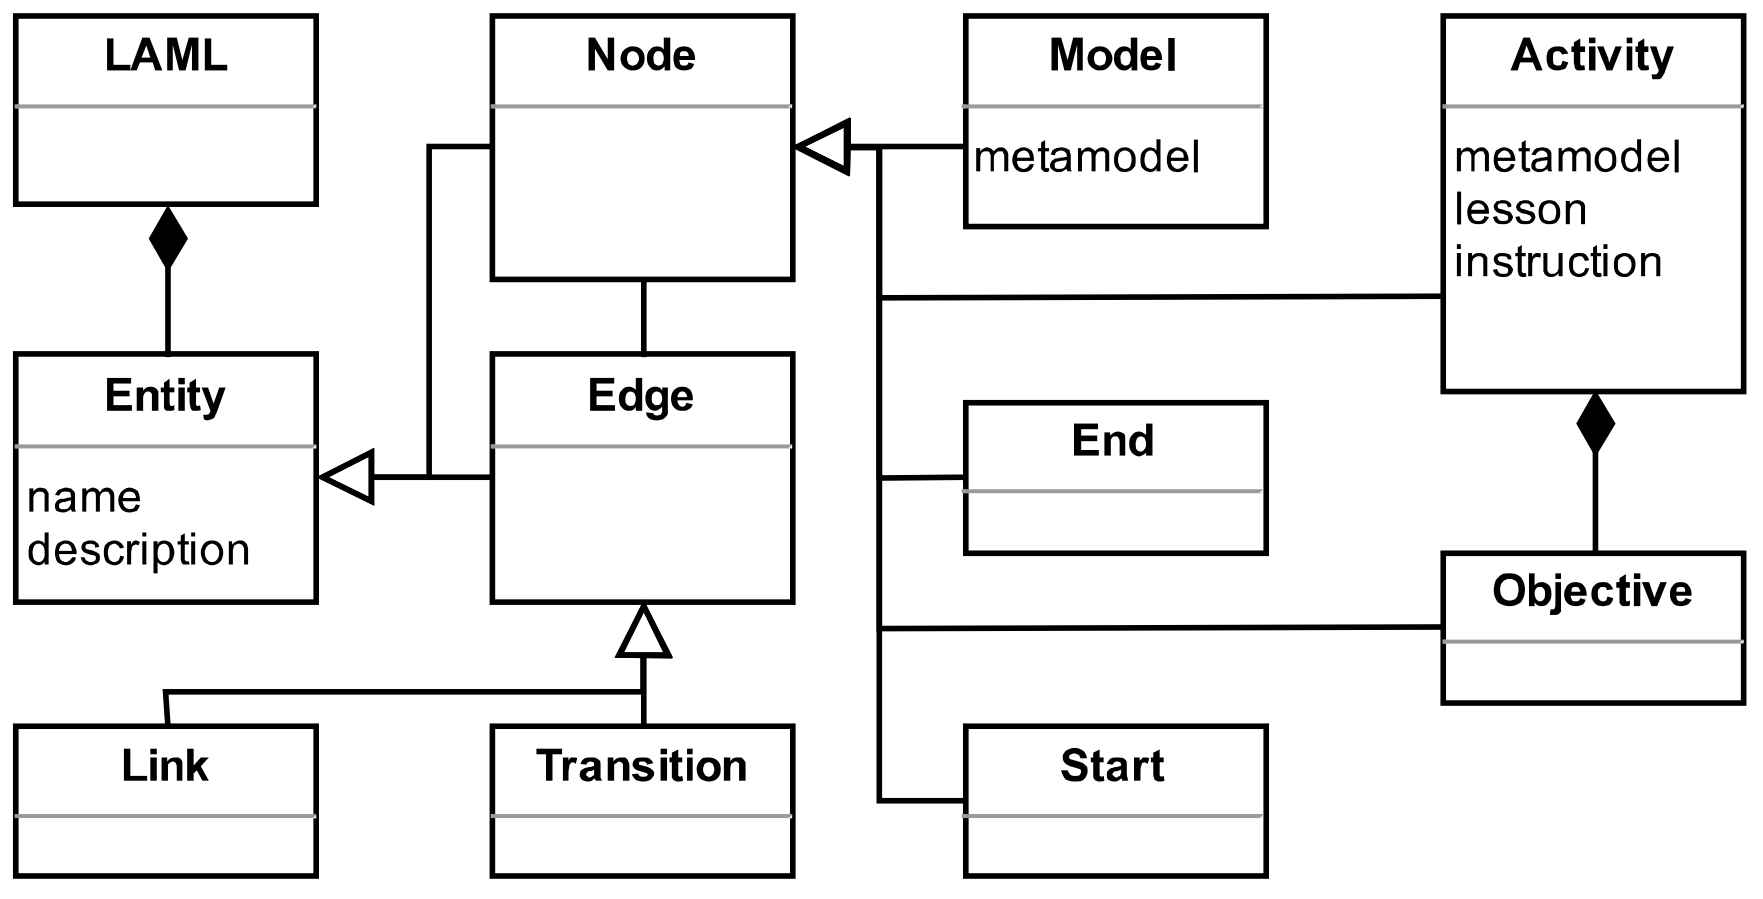
\includegraphics[width=\linewidth]{laml}
\caption{The class diagram of the \emph{learning activity modelling language}.}
\label{laml}
\end{figure}

The statechart diagram is intended to only support six basic elements: state, note, start, end, transition and link. Therefore, six classes are specified to represent the elements (lines 21, 24, 27, 32, 35, 38). State, note, start, and end elements are nodes in the diagram; their classes are derived from Node class, and each is annotated with {\fontfamily{pcr}\selectfont @node}, as well as its MxGraph-related attributes (fillColor, width, height, shape, etc.), to determine its appearance in the diagram (lines 26, 31, 34, 37). Similarly, transition and link are edges in the diagram, extend the Edge class and are annotated with {\fontfamily{pcr}\selectfont @link} (lines 20, 21, 23, 24). The State class has a containment reference named substates that also has type State class. This means that an instance of State class can also contain other instances of State class as its substates. The \emph{substates} attribute is annotated with {\fontfamily{pcr}\selectfont @compartment} which means, in the diagram, a state has a container and other states can be placed inside it to become its substates (lines 28-29). The Node class has two references: outgoing and incoming. Both have the same type, Edge (lines 13-14). The Edge class also has two references: source and target. Both have the same type, Node class (lines 17-18).

\begin{lstlisting}[style=interfaces,caption={A definition of statechart diagram using Emfatic and Eugenia-like annotations.},label=metamodel]
@namespace(uri="statechart", prefix="statechart")
package statechart;

@diagram
class Statechart {
  val Entity[*] entities;
}
abstract class Entity {
  attr String name = "";
  attr String description = "";
}
abstract class Node extends Entity {
  ref Edge[*]#source outgoing;
  ref Edge[*]#target incoming;
}
abstract class Edge extends Entity {
  ref Node#outgoing source;
  ref Node#incoming target;
}
@link(label="name", source="source", target="target", label="name", endArrow="block", blockendFill="1", endSize="6", width="120", height="120")
class Transition extends Edge {
}
@link(label="name", source="source", target="target", label="name", endArrow="none", blockendFill="1", endSize="6", width="120", height="120", dashed="1")
class Link extends Edge {
}
@node(label="name", shape="swimlane", childLayout= "stackLayout", collapsible="1", horizontalStack="0", resizeParent="0", resizeLast="1", rounded="1", marginBottom="7", marginLeft="7", marginRight="7", marginTop="7", whiteSpace="wrap", width="200", height="120", swimlaneFillColor="#FFFFFF")
class State extends Node {
  @compartment(shape="swimlane", collapsible= "0", noLabel="1", editable="0", strokeColor="none", startSize="0")
  val State[*] substates;
}
@node(label="description", shape="note", whiteSpace="wrap", width="200", height="120")
class Note extends Node {
}
@node(label="name", shape="startState", whiteSpace="wrap", fillColor="#000000", width="30", height="30")
class Start extends Node {
}
@node(label="name", shape="endState", whiteSpace="wrap", fillColor="#FFFFFF", width="30", height="30")
class End extends Node {
}
\end{lstlisting} 

\subsection{Create Statechart Model}
Using the generated graphical editor (Fig. \ref{ide}), designers can now create statechart models. The editor has a palette that contains statechart elements which they can drag and drop into a drawing area where they can arrange the elements to construct statechart models. The editor also has a property panel to modify the attributes and appearance of the models. Models that have been created can be saved and loaded again for further operations. The editor also can be used to create models as input/base models for learning activities.        

\begin{figure}[!t]
\centering
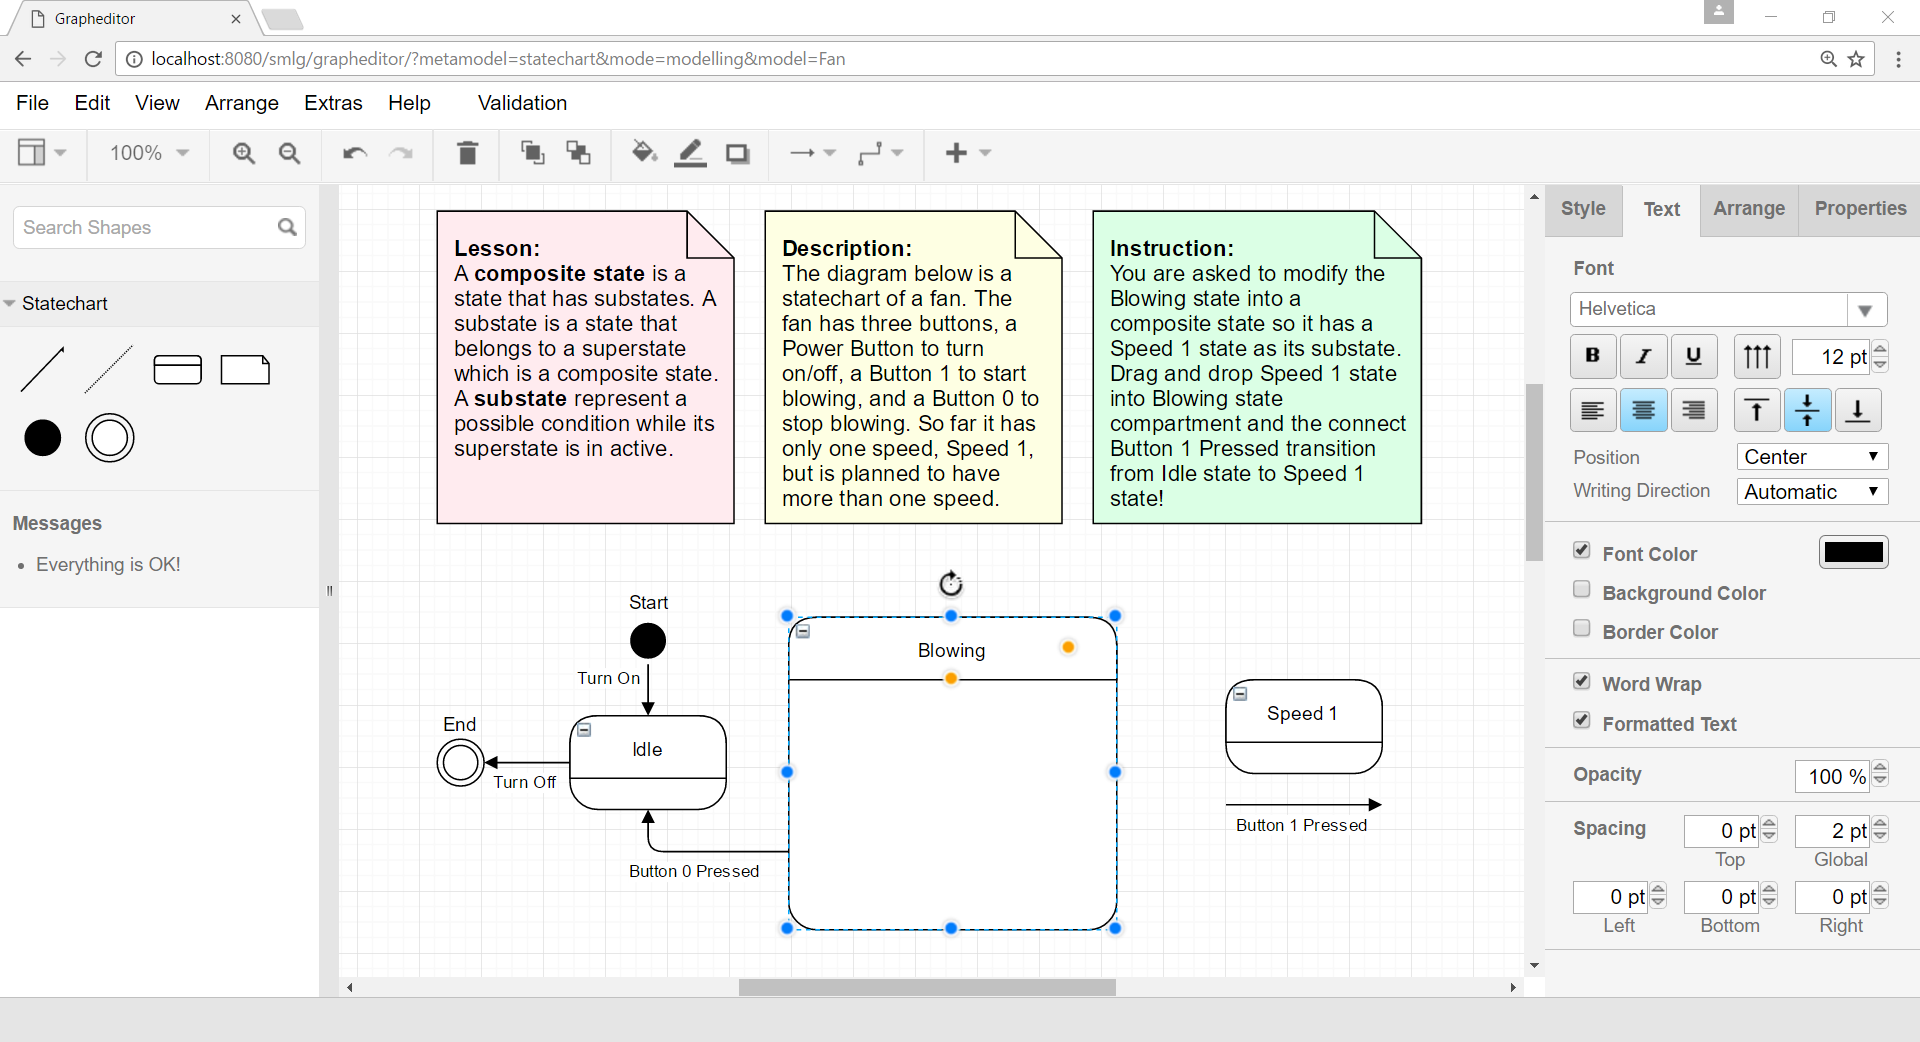
\includegraphics[width=\linewidth]{ide}
\caption{The MxGraph-based graphical editor to create statechart models.}
\label{ide}
\end{figure}

\begin{figure}[!t]
\centering
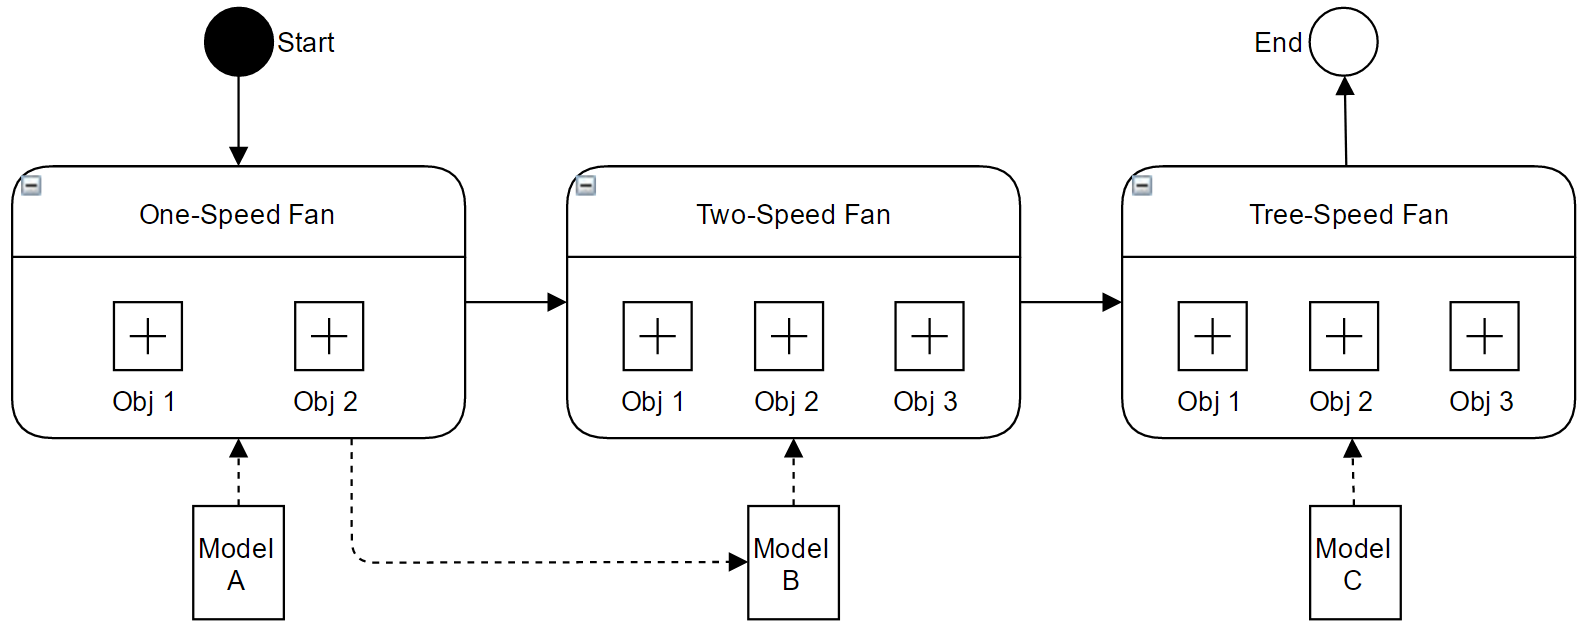
\includegraphics[width=\linewidth]{eoml}
\caption{A learning activity flow for learning the concept of Substates in state-machine modelling.}
\label{eoml}
\end{figure}

\begin{figure}[!t]
\centering
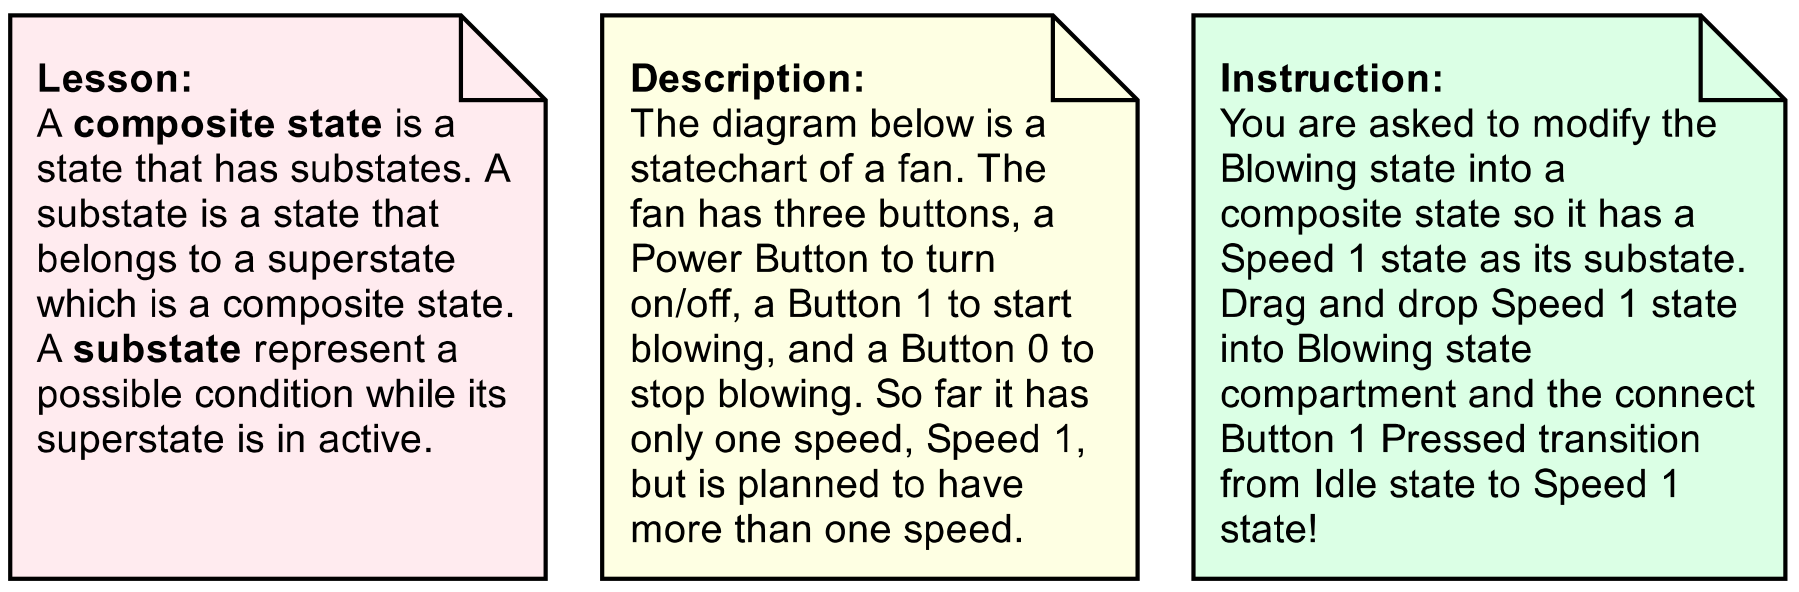
\includegraphics[width=\linewidth]{example-01a}
\caption{Lesson, model description, and instruction.}
\label{example-01a}
\end{figure}

\subsection{Create Learning Activity Model}
To teach a concept, tutors should design learning activities. In this example, a learning activity model to learn the concept of substates is created (Fig. \ref{eoml}). The case is an electrical fan that has two main states, Idle and Blowing. Learners will be asked to modify the Blowing state, so it becomes a composite state with substates that represent the different speeds of blowing. The learning activity has three activities, namely One-Speed Fan, Two-Speed Fan, and Three-Speed Fan. The activities are arranged \textit{per se} to accommodate Flow state \cite{csikszentmihalyi2014toward} so learners can progress from the easiest activity to the hardest one. The activities are explained in more detail in the following subsections.
  
Each activity has a lesson and instruction properties. Lesson contains an explanation of the concepts to be taught; instruction contains commands or questions that learners need to execute or answer. Learners must meet all the objectives of an activity to move to the next activity. Each activity can consume existing models (Model A, B, and C in Fig. \ref{eoml}) as its base models -- so that learners do not have to create models from scratch every time -- and produce a model (Model B in Fig. \ref{eoml}) to be used in its next activity. Each model has a description property, which helps learners to understand about the model. An example of the lesson, model description, and instruction properties of the One-Speed Fan activity (Fig. \ref{eoml}) is displayed in Fig. \ref{example-01a}.    


\subsubsection{One-Speed Fan Activity}
In this activity (Fig. \ref{example-01}), learners are introduced to one substate only. The activity starts with a base model, and learners are required to modify the base model (Fig. \ref{example-01b}) to match the target model (Fig. \ref{example-01c}). The base model corresponds to Model A in Fig. \ref{eoml}, which refers to an existing base model and will be loaded once the activity is executed, so learners do not need to create the model from the start. 

The example case in this activity is a fan that has three buttons, a Power Button to turn on/off, a Button 1 to start blowing, and a Button 0 to stop blowing. So far it has only one speed, Speed 1, but is planned to have more than one speed. Learners are asked to modify the Blowing state in Fig. \ref{example-01b} into a composite state by moving the Speed 1 state into the Blowing state compartment and connecting the Button 1 Pressed transition from the Idle state to the Speed 1 state. Since in Fig. \ref{eoml} this activity is designed to have only two objectives, the two objectives are adjusted and defined as follow: Objective 1 ``The Blowing state contains the Speed 1 substate" and Objective 2 ``Button 1 Pressed transition connects the Idle state to the Speed 1 substate".

\begin{figure}[!t]
    \centering
    \subfloat[Base model]{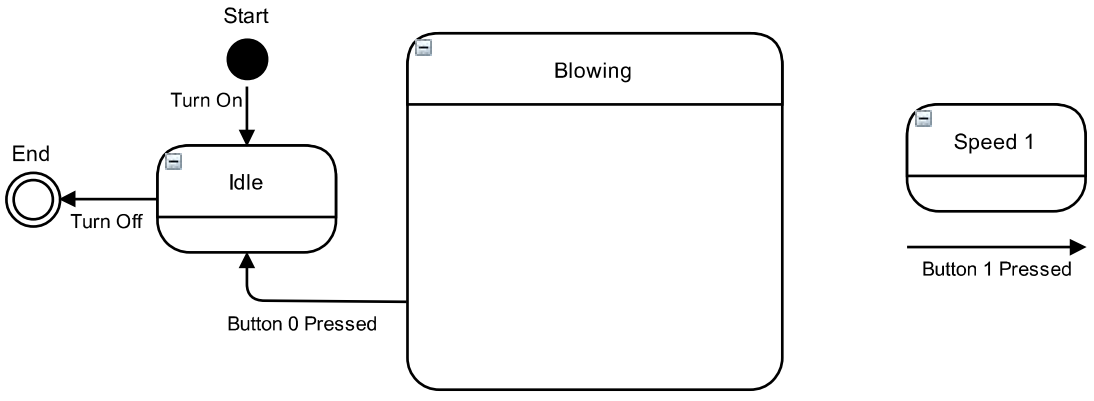
\includegraphics[width=\linewidth]{example-01b}	
    \label{example-01b}}
    \\
    \subfloat[Target model]{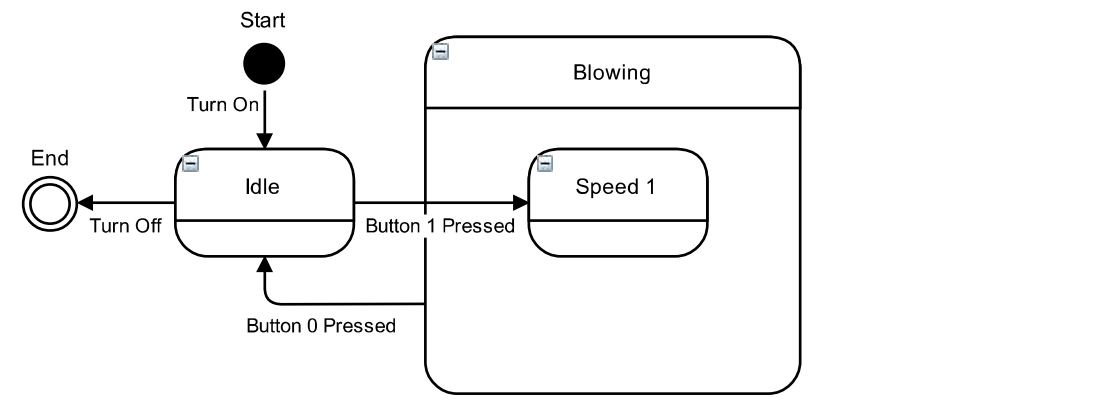
\includegraphics[width=\linewidth]{example-01c}
    \label{example-01c}}
	\caption{The One-Speed Fan example.}
    \label{example-01}
\end{figure}

\begin{figure}[!t]
    \centering
    \subfloat[Base model]{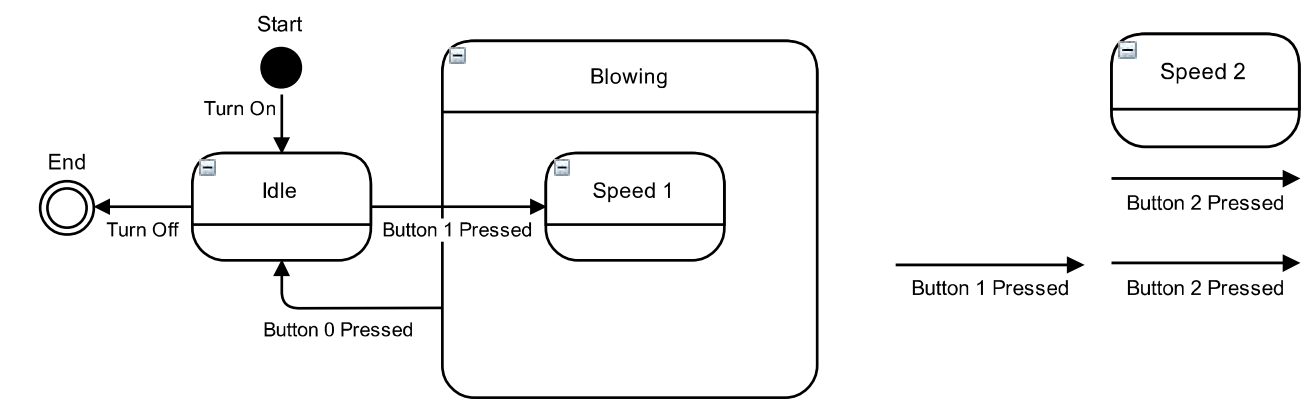
\includegraphics[width=\linewidth]{example-02b}	
    \label{example-02b}}
    \\
    \subfloat[Target model]{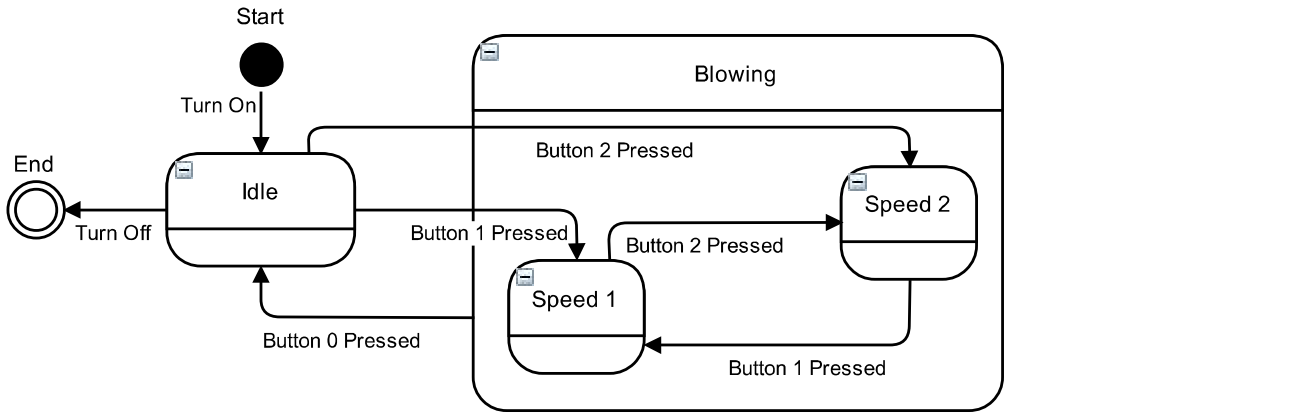
\includegraphics[width=\linewidth]{example-02c}
    \label{example-02c}}
	\caption{The Two-Speed Fan example.}
    \label{example-02}
\end{figure}

\begin{figure}[!t]
    \centering
    \subfloat[Base model]{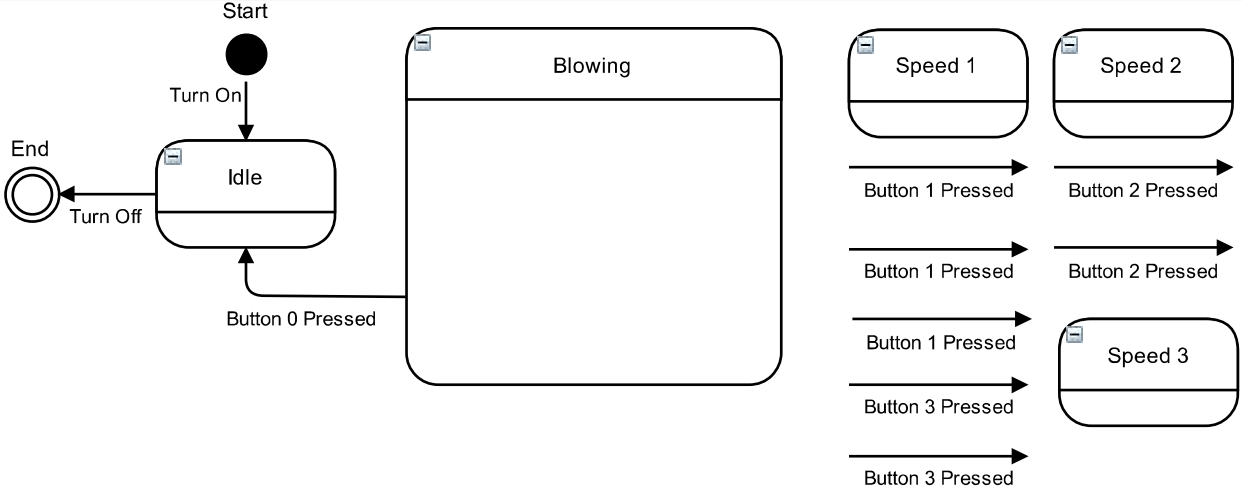
\includegraphics[width=\linewidth]{example-03b}	
    \label{example-03b}}
    \\
    \subfloat[Target model]{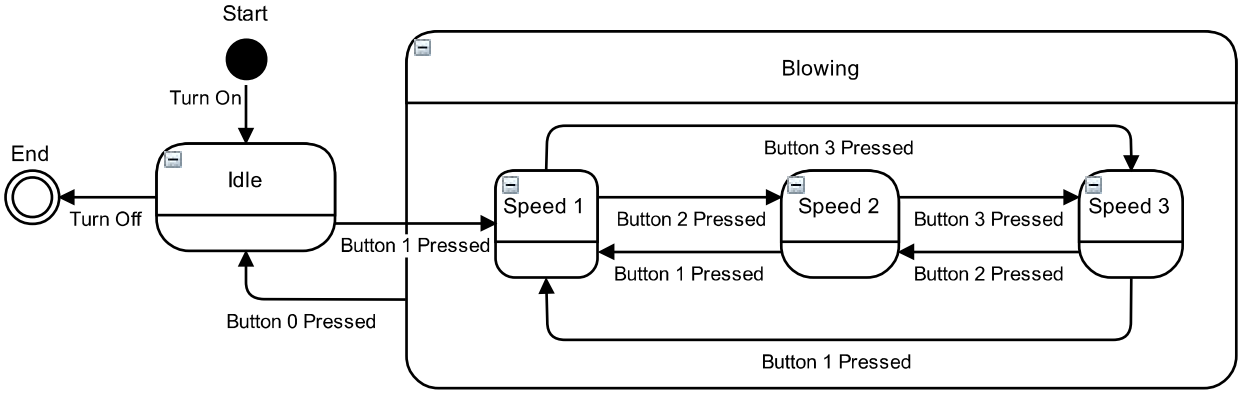
\includegraphics[width=\linewidth]{example-03c}
    \label{example-03c}}
	\caption{The Three-Speed Fan example.}
    \label{example-03}
\end{figure}

\subsubsection{Two-Speed Fan Activity}
The Two-Speed Fan activity (Fig. \ref{example-02}) consumes the model that has been produced in the first activity (Model B in Fig. \ref{eoml}). Any model generated in the previous activity becomes the base model for modelling in this activity. In accordance with the Flow concept \cite{csikszentmihalyi2014toward}, this second activity should be more challenging. Therefore, the activity (Fig. \ref{example-02}) challenges learners with one additional state and three new transitions. Now the case has changed. The fan has an extra button, Button 2, to support 2-speed blowing. When Button 1 is pressed, the fan blows in speed 1 and when Button 2 is pressed, the fan blows in speed 2. Thus, learners need to modify the Blowing state into a composite state, so that it has two-speed states. The fan can move from the Idle state to the Speed 1 state, from the Idle state to the Speed 2 state, and from the Speed 1 state to the Speed 2 state or \textit{vice versa}.

\subsubsection{Three-Speed Fan Activity}
The Three-Speed Fan activity (Fig. \ref{example-03}) should be harder than the second activity. The fan now supports 3 speeds of blowing, but it has been modified so it cannot go directly to Speed 2 or Speed 3 without firstly going to a state with a lower speed. In other words, the transition from Idle can only go to Speed 1 for the fan to start blowing. Thus, starting from the model C as the base model (Fig. \ref{eoml}), learners are required to modify the Blowing state into a composite state with 3 speeds of blowing and to only allow a transition from Idle to Speed 1.

\subsection{Generate Game}
After constructing the learning activity (Fig. \ref{eoml}), designers can now generate a path of levels (or stages). Each generated level corresponds to an activity defined in the learning activity and has an EVL template for validation. The EVL template is shown in Listing \ref{validation-template} which can be extended by designers to write constraints that fit the level scenarios and objectives. The number of constraints and operations in the template corresponds to the number of objectives defined in the level's learning activity activity in Fig. \ref{eoml}. As an example, implementation of validation, Listing \ref{validation-realisation} shows the EVL code to check whether the Blowing state has a Speed 1 substate, as intended by Objective 1 in One-Speed activity.   

\begin{lstlisting}[style=interfaces,caption={Validation template for objectives in One-Speed Fan activity/level.},label=validation-template]
context Statechart {
    constraint obj_1 {
        check: self.obj_1()
        message: "FAIL: ob_1"
    }
    constraint obj_2 {
        check: self.obj_2()
        message:"FAIL: obj_2"
    }        
}
operation Statechart obj_1(): Boolean {
    return true;
}
operation Statechart obj_2(): Boolean {
    return true;
}
\end{lstlisting} 


\begin{lstlisting}[style=interfaces,caption={Validation realisation for Objective 1 in One-Speed Fan activity/level.}, label=validation-realisation]
context Statechart {
    constraint obj_1 {
        check: 
            self.obj_1()
        message:
            "FAIL: Blowing state contains Speed 1 substate"
    }
    ...
}
operation Statechart obj_1(): Boolean {
    return State.all.exists(state | state.name = "Blowing" and state.substates.exists(substate | substate.name = "Speed 1"))
}
...
\end{lstlisting} 

\subsection{Play Game}
After generating the learning activity into a path of ordered levels and defining its levels' validation, learners can choose the path and play its levels as depicted in Fig. \ref{path}. When learners choose the first level, an MxGraph-based editor is displayed and the lesson, model description, instruction, objectives, and base model are presented to learners. Learners can then start to modify the base model to reach the target model. 

\begin{figure}[!t]
\centering
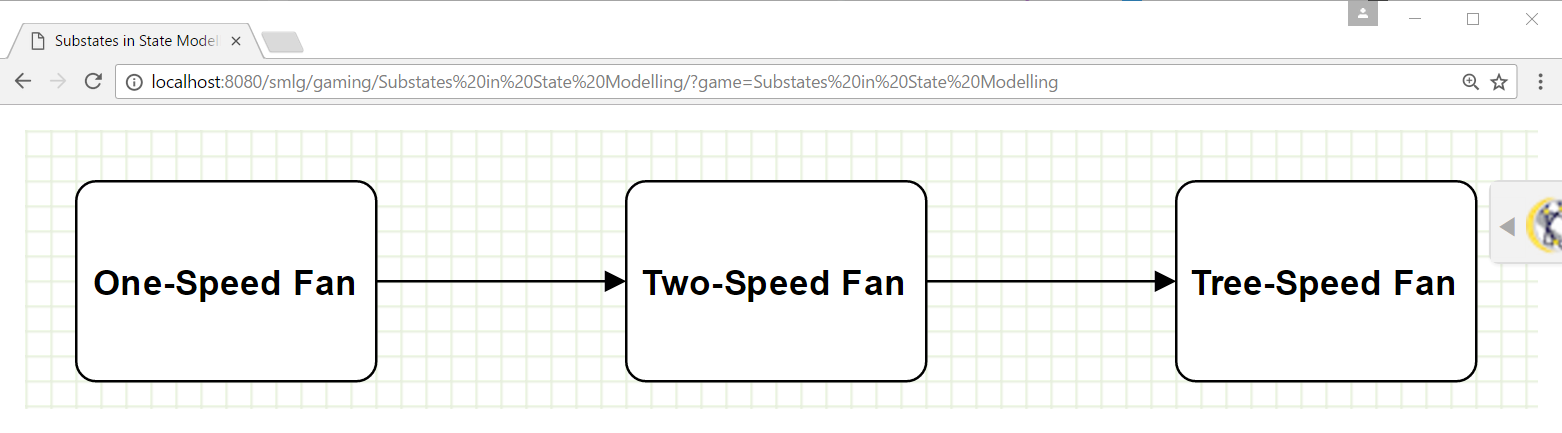
\includegraphics[width=\linewidth]{path}
\caption{The path for learning substate concept with its levels.}
\label{path}
\end{figure}    

Every attempt to change the model triggers an operation to validate the current model using the defined EVL constraints to assess whether the model has met the current level's objectives. If not, feedback is displayed to learners indicating the objectives that have not been satisfied. For example, in Fig. \ref{example-fail-messages}, the Speed 1 substate has not been put into the Blowing state even though the Button 1 Pressed transition has connected the Idle state to the Speed 1 substate. If all objectives have been fulfilled, the level is considered completed, an appropriate message is produced to provide positive reinforcement and the learner can proceed to the next level.  

\begin{figure}[!t]
\centering
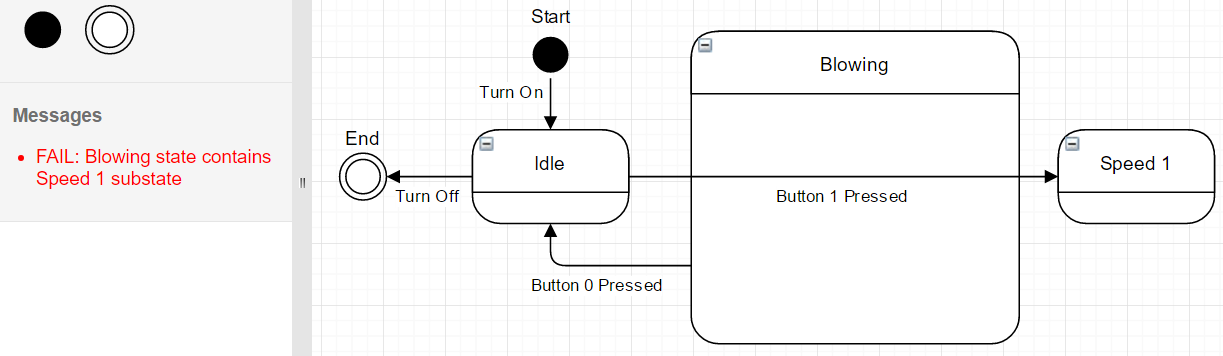
\includegraphics[width=\linewidth]{example-fail-messages}
\caption{A message is displayed to learners indicating the objective that has not been fulfilled.}
\label{example-fail-messages}
\end{figure}  

\section{Evaluation Plans}
\label{Evaluation Plans} 
Two forms of assessment have been planned to evaluate the framework. The first assessment is to measure the effectiveness of modelling games vs. class-based lecturing using controlled experiments involving undergraduate and postgraduate students. Subjects will be grouped into two groups, an experimental group, and a control group. While the control group will only learn from attending class-based lecturing, the other group will also learn using games. Both will be tested with relevant problems before and after teaching to measure their improvement. The gap between the two group will be used to measure the effect of the games. Even though this evaluation is feasible since an adequate number of software engineering students are available, challenges still exist. The quality of the class-based lecturing, the problems given in the tests, and the games should be consistent, ensuring that they carefully designed to address the same educational objectives. The other challenge is to have the two groups of subjects have balanced quality and distribution. 
  
The second assessment is to measure the development effort needed to develop a complete game for a non-trivial modelling language, and the savings realised using the model-driven approach. The assessment will be tested on developers that have considerable background in developing games, which also implies a challenge since it is difficult to get developers that have such qualification and are willingly participate as subjects. The measures will be on time used to complete the game and ratio between lines of code written and lines of code generated. Subjective feedback from the developers will also be useful to describe the quality of the framework.  
  
\section{Related Work}
\label{Related Work}
There are not many studies that investigate the application of gameful approaches in software modelling. Stikkolorum et al. \cite{Stikkolorum2014} develop a game that is intended to teach software design principles, such as cohesion, coupling, information hiding, and modularity in object-oriented software design. Groenewegen et al. \cite{Groenewegen2010} apply gamification to improve stakeholders' understanding of their enterprise architecture models as well as to validate them. In the domain of information security modelling, Ionita et al. \cite{Ionita2015} develop a socio-technical modelling language (TREsPASS) that maps information on security-related concepts toward familiar, physical representation to ease interaction and undestanding. In the context of activity diagram learning, Richardsen \cite{Richardsen2014} develops a game, whose behaviours are controlled through a UML activity diagram. De Smedt et al. \cite{de2015gamification} gamify Declare models using the guessing mechanism supported by annotation of constraint, dependency information, and feedback, so players are more informed and engaged in constructing the models. Unlike our approach which attempts to offer a reusable gamification framework, each study addresses a different topic in software modelling using different approaches and game elements. Common drawbacks of the studies are that most of them do not consider the pedagogical aspect of their solution, and their validation is weak in sample size as well as the lack of discussion of internal validity.

\section{Conclusions}
\label{Conclusions}
In this paper, we have proposed a framework for model-driven gamified software modelling learning---a framework that combines the engaging nature of games, effectiveness of pedagogy, and automation of Model-Driven Engineering. It is a framework for tutors to construct software modelling learning activities, which then uses model transformation to produce software modelling learning games. The motivation behind the framework has been presented, as well as the problem analysis, and an overview of the framework have been explained. The framework also has been demonstrated, and its evaluation approach has been proposed.

In the future, we plan to add, (1) a fine-grained logging framework that will allow game designers to replay solutions and understand how users interact with the game. (2) an automated model mutation facility to automatically generate incorrect alternatives in levels with multiple-choice gameplay. (3) a facility that monitors the progress of learners and adapts the game accordingly (e.g. displays fewer instructions, allows fast learners to skip levels, or recommends other related games to play).

% An example of a floating figure using the graphicx package.
% Note that \label must occur AFTER (or within) \caption.
% For figures, \caption should occur after the \includegraphics.
% Note that IEEEtran v1.7 and later has special internal code that
% is designed to preserve the operation of \label within \caption
% even when the captionsoff option is in effect. However, because
% of issues like this, it may be the safest practice to put all your
% \label just after \caption rather than within \caption{}.
%
% Reminder: the "draftcls" or "draftclsnofoot", not "draft", class
% option should be used if it is desired that the figures are to be
% displayed while in draft mode.
%
%\begin{figure}[!t]
%\centering
%\includegraphics[width=2.5in]{myfigure}
% where an .eps filename suffix will be assumed under latex, 
% and a .pdf suffix will be assumed for pdflatex; or what has been declared
% via \DeclareGraphicsExtensions.
%\caption{Simulation results for the network.}
%\label{fig_sim}
%\end{figure}

% Note that the IEEE typically puts floats only at the top, even when this
% results in a large percentage of a column being occupied by floats.


% An example of a double column floating figure using two subfigures.
% (The subfig.sty package must be loaded for this to work.)
% The subfigure \label commands are set within each subfloat command,
% and the \label for the overall figure must come after \caption.
% \hfil is used as a separator to get equal spacing.
% Watch out that the combined width of all the subfigures on a 
% line do not exceed the text width or a line break will occur.
%
%\begin{figure\\}[!t]
%\centering
%\subfloat[Case I]{\includegraphics[width=2.5in]{box}%
%\label{fig_first_case}}
%\hfil
%\subfloat[Case II]{\includegraphics[width=2.5in]{box}%
%\label{fig_second_case}}
%\caption{Simulation results for the network.}
%\label{fig_sim}
%\end{figure\\}
%
% Note that often IEEE papers with subfigures do not employ subfigure
% captions (using the optional argument to \subfloat[]), but instead will
% reference/describe all of them (a), (b), etc., within the main caption.
% Be aware that for subfig.sty to generate the (a), (b), etc., subfigure
% labels, the optional argument to \subfloat must be present. If a
% subcaption is not desired, just leave its contents blank,
% e.g., \subfloat[].


% An example of a floating table. Note that, for IEEE style tables, the
% \caption command should come BEFORE the table and, given that table
% captions serve much like titles, are usually capitalized except for words
% such as a, an, and, as, at, but, by, for, in, nor, of, on, or, the, to
% and up, which are usually not capitalized unless they are the first or
% last word of the caption. Table text will default to \footnotesize as
% the IEEE normally uses this smaller font for tables.
% The \label must come after \caption as always.
%
%\begin{table}[!t]
%% increase table row spacing, adjust to taste
%\renewcommand{\arraystretch}{1.3}
% if using array.sty, it might be a good idea to tweak the value of
% \extrarowheight as needed to properly center the text within the cells
%\caption{An Example of a Table}
%\label{table_example}
%\centering
%% Some packages, such as MDW tools, offer better commands for making tables
%% than the plain LaTeX2e tabular which is used here.
%\begin{tabular}{|c||c|}
%\hline
%One & Two\\
%\hline
%Three & Four\\
%\hline
%\end{tabular}
%\end{table}


% Note that the IEEE does not put floats in the very first column
% - or typically anywhere on the first page for that matter. Also,
% in-text middle ("here") positioning is typically not used, but it
% is allowed and encouraged for Computer Society conferences (but
% not Computer Society journals). Most IEEE journals/conferences use
% top floats exclusively. 
% Note that, LaTeX2e, unlike IEEE journals/conferences, places
% footnotes above bottom floats. This can be corrected via the
% \fnbelowfloat command of the stfloats package.



% conference papers do not normally have an appendix


% use section\\ for acknowledgment
\section*{Acknowledgments}
This research is part of a doctoral programme funded by \emph{Lembaga Pengelola Dana Pendidikan Indonesia} (Indonesia Endowment Fund for Education).

% trigger a \newpage just before the given reference
% number - used to balance the columns on the last page
% adjust value as needed - may need to be readjusted if
% the document is modified later
%\IEEEtriggeratref{8}
% The "triggered" command can be changed if desired:
%\IEEEtriggercmd{\enlargethispage{-5in}}

% references section

% can use a bibliography generated by BibTeX as a .bbl file
% BibTeX documentation can be easily obtained at:
% http://mirror.ctan.org/biblio/bibtex/contrib/doc/
% The IEEEtran BibTeX style support page is at:
% http://www.michaelshell.org/tex/ieeetran/bibtex/
%\bibliographystyle{IEEEtran}
% argument is your BibTeX string definitions and bibliography database(s)
%\bibliography{IEEEabrv,../bib/paper}
%
% <OR> manually copy in the resultant .bbl file
% set second argument of \begin to the number of references
% (used to reserve space for the reference number labels box)
%\begin{thebibliography}{1}
%
%\bibitem{IEEEhowto:kopka}
%H.~Kopka and P.~W. Daly, \emph{A Guide to \LaTeX}, 3rd~ed.\hskip 1em plus
%  0.5em minus 0.4em\relax Harlow, England: Addison-Wesley, 1999.
%
%\end{thebibliography}

\bibliographystyle{IEEEtran}
\bibliography{references}



% that's all folks
\end{document}